% !TEX root = ./rapport.tex

\section{Interface graphique}

\subsection{Menu principal}

\begin{figure}[htbp]
    \centering
    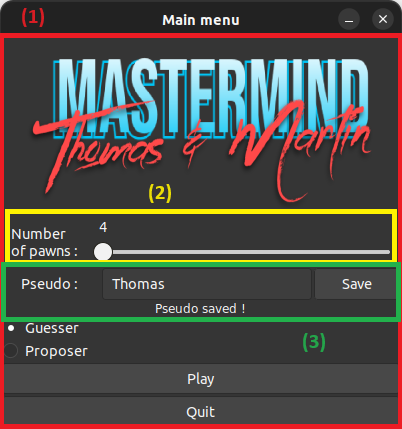
\includegraphics[width=0.5\textwidth]{main_menu.png}
    \caption{Fenêtre du menu principal.}
\end{figure}

La fenêtre du menu principal se décompose en une box verticale principale $(1)$ qui contient :
\begin{itemize}
    \item l'image du logo,
    \item $(2)$ une première box horizontale contenant le label $"Number~of~ pawns"$ ainsi que le slider permettant de sélectionner le nombre de pions de la partie (entre 4 et 8),
    \item $(3)$ une deuxième box horizontale contenant le label $"Pseudo:"$, une boite d'entrée de texte permettant au joueur de rentrer son pseudo ainsi qu'un bouton $Save$ pour le sauvegarder,
    \item un message informant de la validité et de la bonne sauvegarde du pseudo,
    \item deux boutons permettant de choisir le rôle de $Guesser$ (le joueur devine la combinaison aléatoire de l'ordinateur) ou $Proposer$ (l'ordinateur devine la combinaison du joueur),
    \item un bouton $Play$ permettant de lancer une partie,
    \item un bouton $Quit$ permettant de quitter le jeu.
\end{itemize}

\subsection{Jeu}

\begin{figure}[htbp]
    \centering
    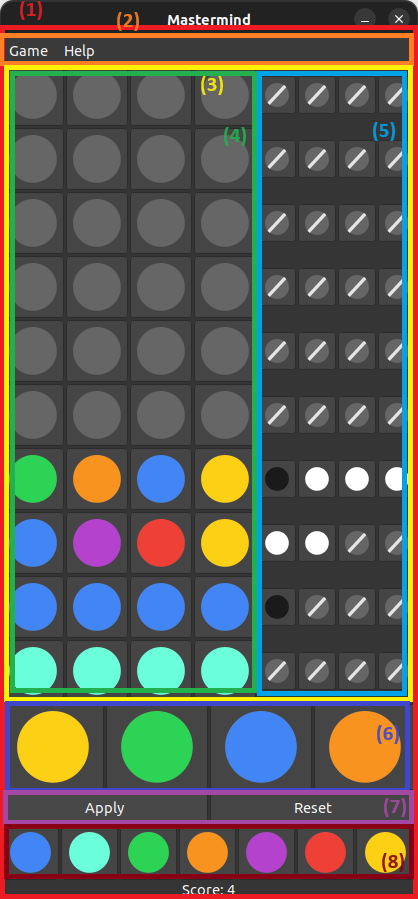
\includegraphics[width=0.414\textwidth]{game_guesser.png}
    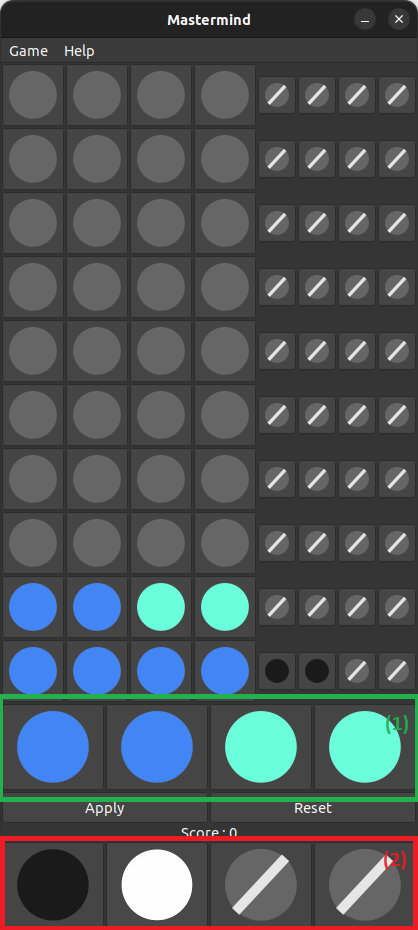
\includegraphics[width=0.4\textwidth]{game_proposer.png}
    \caption{Fenêtres de jeu ($Guesser$ à gauche et $Proposer$ à droite).}
\end{figure}

Les fenêtres de jeu en mode $Guesser$ et $Proposer$ partagent des éléments similaires. Les boites allant de $(1)$ à $(5)$ sur l'image de la fenêtre du jeu en mode $Guesser$ seront uniquement définies pour le mode $Guesser$ mais fonctionnent de la même manière en mode $Proposer$.
\\\\
La fenêtre de jeu se décompose en une box verticale principale $(1)$ contenant :

\begin{itemize}
    \item $(2)$ une barre de menu avec un bouton $Game$ et un bouton $Help$. $Game$ donne accès à un menu déroulant permettant les choix :
    \begin{itemize}
        \item $Main Menu$ qui permet de retourner au menu principal,
        \item $Score$ qui affiche une fenêtre répertoriant les 10 scores les plus élevés enregistrés,
        \item $Quit$ qui quitte complètement le jeu.
    \end{itemize}
    \item $(3)$ une table $Gtk$ organisant les boutons des boîtes $(4)$ et $(5)$. Il s'agit de l'historique de la partie.
    \item $(4)$ une matrice de boutons servant à l'affichage des images des pions de couleur. Ces lignes de boutons représentent les combinaisons proposées.
    \item $(5)$ une matrice de boutons servant à l'affichage des images des pions de feedback. Ces lignes de boutons sont les résultats correspondants aux combinaisons.
    \item[]
\end{itemize}

En mode de jeu $Guesser$, le tableau de boutons $(6)$ permet au joueur de créer une combinaison grâce aux différentes couleurs du tableau de boutons $(8)$. Une fois satisfait de la combinaison crée, le joueur peux proposer sa combinaison à l'aide du bouton $Apply$ $(7)$. Dans le cas contraire, le bouton $Reset~(7)$ permettera au joueur d'effacer sa combinaison. 
\\\\
En mode de jeu $Proposer$, l'affichage est, dans un premier temps, identique à celui du mode $Guesser$. Pour créer la combinaison que l'ordinateur devra trouver, le joueur utilise le même système que celui permettant de proposer des combinaisons en mode $Guesser$. Une fois la combinaison secrète proposée, elle est conservée dans la zone $(1)$ (sur l'image de la fenêtre du jeu en mode $Proposer$). Dès lors, l'ordinateur propose une combinaison qui est affichée dans l'historique et le joueur donne le résultat de la combinaison grâce aux boutons de la zone $(2)$. Pour faire apparaître des pions noirs ou blancs, le joueur devra cliquer plusieurs fois sur les boutons. Lorsque ce dernier est certain du résultat qu'il va donner à l'ordinateur, il le soumet via le bouton $Apply$.

\begin{figure}[htbp]
    \centering
    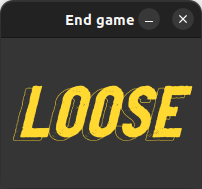
\includegraphics[width=0.2\textwidth]{loose.png}
    \caption{Fenêtre pop-up perdant.}
\end{figure}
En fin de jeu, une fenêtre pop-up apparaît affichant le résultat de la partie. Nous vous laissons le plaisir de découvrir l'affichage gagnant en ne vous dévoilant que le perdant.